\documentclass[a4paper]{article}
\usepackage{graphicx}
\usepackage{xcolor}
\usepackage{url}
\usepackage{outlines}
\usepackage{listings}
\usepackage{fontspec}
\lstset{basicstyle=\ttfamily,
	showstringspaces=false,
	commentstyle=\color{blue},
	keywordstyle=\color{pink}
}
\lstset{emph={
	EXPOSE,RUN,FROM,CMD,nc,tcp,udp,http,docker},emphstyle=\color{purple}
}
\newcommand{\abc}{\hfill \break}
\newcommand{\ii}{\textit}
\usepackage{fancyhdr}
\usepackage{geometry}
% \usepackage{hyperref}
% \hypersetup{
% 	colorlink=true,
% 	linktoc=all,
% 	linkcolor=pink,
% }
\geometry{
	a4paper,
	total={170mm,257mm},
	left=20mm,
	top=20mm,
	bottom=39mm,
}

\setlength{\headheight}{82.70538pt}

\fancypagestyle{oida}{
	\fancyhf{}
	\fancyhead[L]{\fontsize{7.5}{7.5}htl donaustadt\\ Donaustadtstraße 45\\
		1220 Wien\\~\\ Abteilung: Informationstechnologie\\ 
	Schwerpunkt: Netzwerktechnik}
	\fancyhead[R]{
\includegraphics[scale=0.45]{images/logo.png}}

	\fancyfoot[L]{\today}
	\fancyfoot[C]{\jobname}
	\fancyfoot[R]{Seite: \thepage}
}

\begin{document}
\pagestyle{oida}
\section*{Configure Basic Router Settings}
\par\noindent\rule{\textwidth}{0.4pt}

Laboratory protocol
Configure Basic Router Settings

\begin{figure}[h]
	
\includegraphics[scale=0.2]{images/mika.jpeg}
	\centering
\end{figure}

\vspace*{\fill}
Subject:	NWT|ANGE

Class:	3AHITN

Name:	Stefan Fürst, Marcel Raichle

Group Name/Number: Dumm und Dümmer/7

Supervisor: 	ANGE

Exercise dates:	

Submission date:


\newpage
\tableofcontents

\newpage

\section{Task definition}



\section{Summary}

\newpage

\section{Complete network topology of the exercise}
\section{TODO ADD IP ADDRESSES TO THE TOPOLOGY}
\begin{figure}[h]
	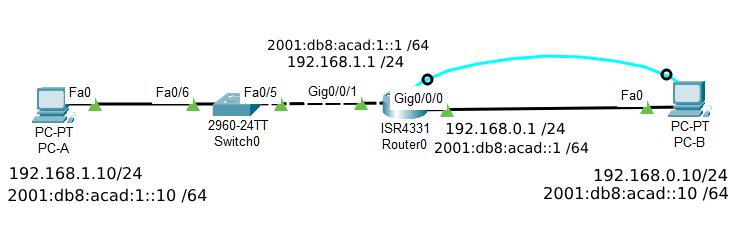
\includegraphics[scale=0.65]{images/nwtopology2.png}
	\centering
	\caption{Complete network topology of this exercise}
\end{figure}

\newpage

\section{Exercise Execution}
\subsection{Set Up the Topology and Initialize Devices}
This exercise was done in Cisco Packet Tracer and the devices were placed and wired using the automatic cabling type, as all the devices are Auto-MDIX compliant anyway.\abc
\begin{figure}[h]
	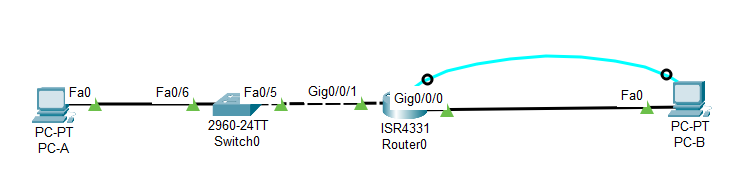
\includegraphics[scale=0.45]{images/nwtopology.png}
	\centering
	\caption{Network topology required for this exercise}
\end{figure}\abc
After that, everything was turned on and the router and switch were both iniliazised and reloaded.

\subsection{Configure Devices and Verify Connectivity}
\subsubsection{Configure the PC interfaces}
The IP addresses for both PCs have been set in the IP Configuration application.
\begin{figure}[h]
	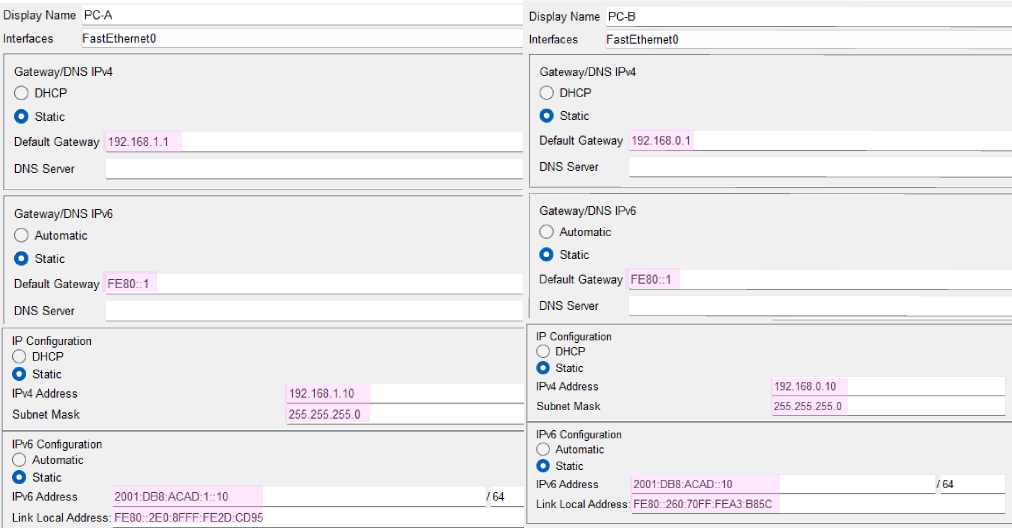
\includegraphics[scale=0.45]{images/pc-ipconf.png}
	\centering
	\caption{IP configuration for PC-A and PC-B}
\end{figure}
\newpage
\subsection{Configure the router}
To access the router's configuration mode, connect to the router through the console port and execute the \ii{en} and \ii{conf t} commands.\abc
The following basic settings are configured using the commands listed below:
\begin{lstlisting}[language=bash,
	keywordstyle=\color{black},
	rulecolor=\color{blue}]
#setting the hostname
hostname R1
#setting the domain name of the router
ip domain name ccna-lab.com
#disable DNS lookup on mistyped commands
no ip domain lookup
#encrypt plain text passwords
service password-encryption
#setting the minimum password length to 12 characters
security passwords min-length 12
\end{lstlisting}
To set up SSH for configuring the router over the network, first, a user must be created with the \ii{username SSHadmin secret 55Hadm!n2020} command, which creates a user named SSHadmin and sets an encrypted password.\abc
Once the user has been created, an RSA key pair needs to be generated using the \ii{crypto key generate rsa general-keys modulus 1024}\footnote{As this is done in Packet Tracer and the hardware in the lab is outdated, the keys are limited to 1024 bit length instead of the 4096 bit length that should be used in a production environment.} command.

\begin{figure}[h]
	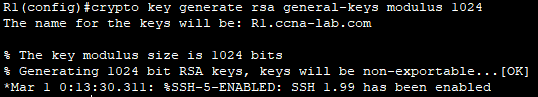
\includegraphics[scale=0.55]{images/keygen.png}
	\centering
	\caption{Key pair generation}
\end{figure}
\begin{lstlisting}[language=bash,
	keywordstyle=\color{black},
	rulecolor=\color{blue}]
#setting a password to enter EXEC mode
enable secret $cisco!PRIV*
line console 0
#setting password for console access
password $cisco!!CON*
#termination of the session after four minutes of inactivity
exec-timeout 4 0
#enabeling login 
login
\end{lstlisting}
\begin{figure}[h]
	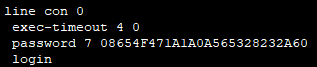
\includegraphics[scale=0.55]{images/line con0.png}
	\centering
	\caption{Viewing the configuration of VTY line 0}
\end{figure}
\begin{lstlisting}[language=bash,
	keywordstyle=\color{black},
	rulecolor=\color{blue}]
#entering the configuration for lines for vty lines 0 to 4
line vty 0 4
#setting a password to access the lines
password $cisco!!VTY*
#termination of the session after four minutes of inactivity
exec-timeout 4 0
#only allowing ssh connections
transport input ssh
#enabeling login using the local database
login local
\end{lstlisting}
\begin{figure}[h]
	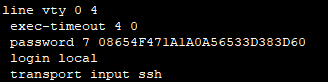
\includegraphics[scale=0.55]{images/votylines.png}
	\centering
	\caption{Viewing the configuration of VTY lines 0 4}
\end{figure}
\begin{lstlisting}[language=bash,
	keywordstyle=\color{black},
	rulecolor=\color{blue}]
#createing a banner to warn that unauthorized access is prohibited
banner motd $ unauthorized access is prohibited $
\end{lstlisting}
\begin{figure}[h]
	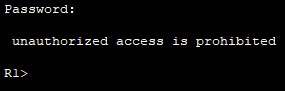
\includegraphics[scale=0.55]{images/banner.png}
	\centering
	\caption{Viewing the MOTD banner}
\end{figure}\abc

\begin{lstlisting}[language=bash,
	keywordstyle=\color{black},
	rulecolor=\color{blue}]
#enable ipv6 routing
ipv6 unicast-routing
#setting the ip addresses according to the addressing table
interface g0/0/0
ip address 192.168.0.1 255.255.255.0
ipv6 address fe80::1 link-local
ipv6 address 2001:db8:acad::1/64
no shutdown
exit
interface g0/0/1
ip address 192.168.1.1 255.255.255.0
ipv6 address fe80::1 link-local
ipv6 address 2001:db8:acad:1::1/64
no shutdown
exit
interface loopback0
ip address 10.0.0.1 255.255.255.0
ipv6 address fe80::1 link-local
ipv6 address 2001:db8:acad:2::1/64
no shutdown
exit
\end{lstlisting}
\newpage
\begin{figure}[h]
	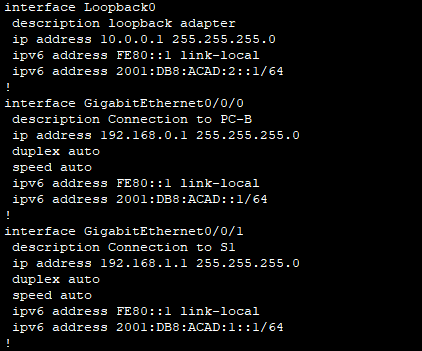
\includegraphics[scale=0.55]{images/showip.png}
	\centering
	\caption{Displaying the IP addresses set}
\end{figure}
\begin{lstlisting}[language=bash,
	keywordstyle=\color{black},
	rulecolor=\color{blue}]
#setting a timeout of 2 minutes after 3 failed login attempts in 60 seconds
login block-for 120 attempts 3 within 60
exit
#setting the clock
clock set 9:22:40 08 Nov 2024
\end{lstlisting}
\begin{figure}[h]
	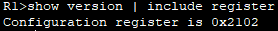
\includegraphics[scale=0.55]{images/showclock.png}
	\centering
	\caption{Display of current time}
\end{figure}\abc

\begin{lstlisting}[language=bash,
	keywordstyle=\color{black},
	rulecolor=\color{blue}]
#copying the current running-config to the startup-config
copy run start
\end{lstlisting}
If the router is reloaded before running this command, the running configuration will be lost, as the RAM is erased during a reload.
\subsection{Verify network connectivity}

\newpage
\section{List of figures}

\listoffigures

\end{document}
